\section{Implementation}\label{sec:implementation}

\subsection{Feed-Forward Neural Network}

Feed-forward networks, otherwise referred to as multi-layer perceptrons, have three primary components: an input layer, zero-to-many hidden layers, and an output layer \citep{Fine1999}. Each layer contains a set of neurons which interact with an input vertex via a weighting vertex and activation function (Figure 2.1). For our implementation, the input layer has been abstracted such that it does not actually contain any neurons. Neurons in the hidden layers apply weights to the input vector, which is then passed to a logistic activation function (Equations 1 and 2).

\begin{equation}
a_h = w^T_h\hat{x}
\end{equation}

Where $w^T_h$ is the weight vector for neuron $h$, and $\hat{x}$ is the input vector $\{x_1, x_2, ..., x_M\}$. From the created value $a_h$, hidden layer neurons can then calculate their output values $z_h$.

\begin{figure}[b!]
	\centering
	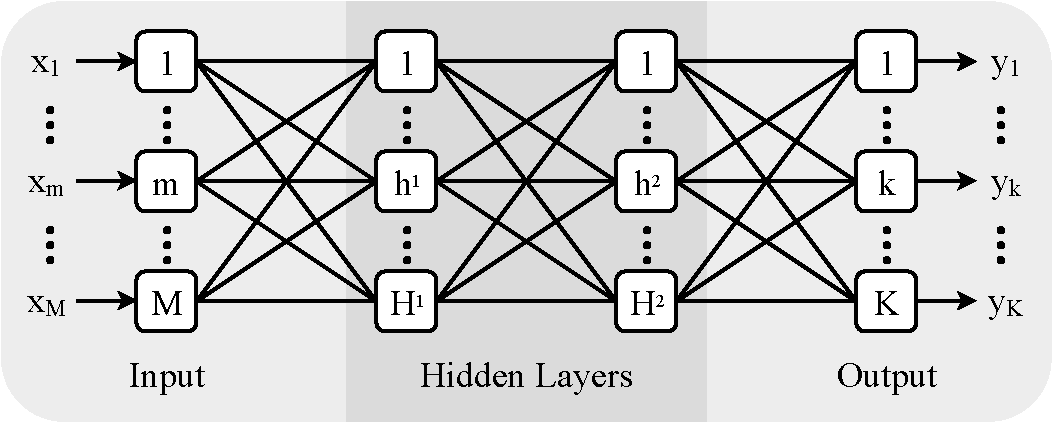
\includegraphics[width=0.9\linewidth]{images/feed_forward_diagram.pdf}
	\caption{Generic diagram of a feed-forward network with two hidden layers, where there are $M$, $H_1$, $H_2$, and $K$ neurons in each layer.}
\end{figure}

\begin{equation}
z_h = \frac{1}{1 + \text{exp}\left({-a_h}\right)}
\end{equation}

\bigbreak
If the network is used for a classification set, the output layer will also use this method for generating its outputs (where there will be an output neuron for each $k$ possible classifications, where the largest output determines the classification of the input) whereas regression sets will use a single linear activation function, which simply returns $y_k = a_k = w^T_k\hat{x}$ as an estimation of the actual value of the input.

When training a feed-forward network, our model takes in a training set, and then performs forward propagation, followed by back propagation. In forward propagation, the first layer takes in the features of the training row, then each proceeding layer takes in a vector of the previous layer's results until reaching the output layer. The resulting vector of the output layer is the result of forward propagation. We then perform back propagation using this result, where we calculate a change in weighting values using stochastic gradient descent. For this, we have two cost functions which correspond to the output layer (Equation 3) and all preceding layers (Equation 4):

\begin{equation}
	\delta_k = r_k - y_k
\end{equation}
\begin{equation}
	\delta_h = z_h(1 - z_h)\mathlarger{\mathlarger{\Sigma}}_{_i}(\delta_i)
\end{equation}

\bigbreak
Where $\delta_i$ is the cost for the $i$th neuron in the following layer and $r_k$ is the expected output for a given output neuron $k$. For categorization, $r_k$ is 1 if the input values are from the class of the corresponding output neuron and 0 otherwise, while $r_k$ is the actual value of the input entry in regression sets. For each neuron $n$ in the network, their weights are then updated using the following equations:

\begin{equation}
\Delta_i = (\eta\delta_i)\hat{x}
\end{equation}
\begin{equation}
	w_i = w_i + \Delta^\phi_i + \alpha\Delta^{\phi - 1}_i
\end{equation}

\bigbreak
Where $\eta$ and $\alpha$ are tuned constants which correspond to the learning rate and momentum of the network, and $\phi$ is the current iteration of back propagation. The learning rate is used to dampen the impact of the changes made, so that any given category being trained is not over-emphasized during classification, while momentum is used to add a portion of the previous epoch of back propagation onto the current changes, such to continue a 'trend' towards an optimized weight.

Back propagation is then repeated until convergence (when the output of the network ceases to change on further iterations) or until an arbitrary loop threshold has been met. Once this process of forward and back propagation has been repeated for every entry in the training dataset, the network is considered 'trained' and can be used to classify new inputs.

\subsection{Radial Basis Function Neural Network}

Radial basis function (RBF) networks operate similarly to feed forward networks, with an input layer, intermediary layer, and output layer. The notable difference between the two networks is that in and RBF network there is always one layer between the input and output layers (Figure 2.2)\citep{Fernandez2012}. Neurons in the intermediary layer also use a radial basis function rather than a sigmoid function for activation. For our purposes, neurons in our implementation use a Gaussian basis function (Equation 7).

\begin{figure}[t!]
	\centering
	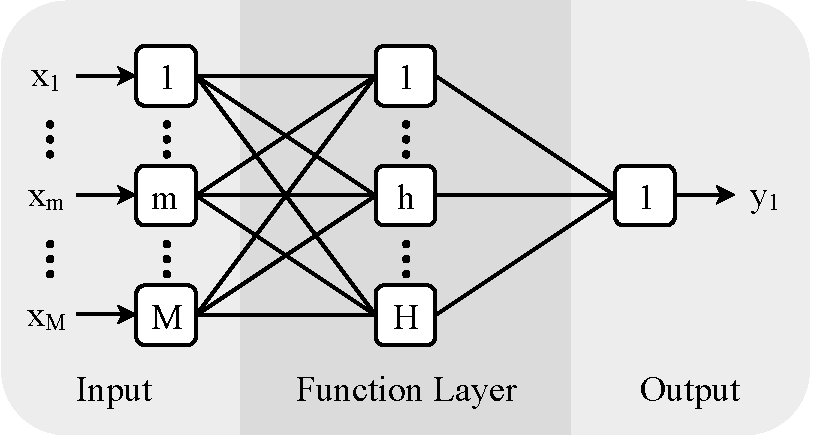
\includegraphics[width=0.7\linewidth]{images/radial_basis_function_diagram.pdf}
	\caption{Generic radial basis function (RBF) neural network with $M$ inputs, $H$ Gaussian basis function neurons, and one output neuron.}
\end{figure}

\begin{equation}
z_h = \text{exp}{\left(-\frac{(\|\hat{x} - c_h\|)^2}{r^2_h}\right)}
\end{equation}

Where $c_h$ is the 'center' -- or prototype -- of the neuron $h$, and $r_h$ is the kernel width of the neuron's function. The $c_h$ of each neuron is determined using the values of the training set passed to the network, while the $r_h$ is calculated using the distance between the function's center and its closest neighbor (Equation 8)\citep{Nabil2003}.

\begin{equation}
	r = ||c_n - c_h||
\end{equation}

Where $c_n$ is the center of the center of the nearest neighbor to $c_h$.

There are several methods for selecting the centers and number of neurons, each of which relies on reducing the initial training dataset into a smaller essential training set. For our purposes, we applied three of these methods: condensed nearest neighbor, k-means clustering, and partitioning around medoids.

\subsubsection{The k-Nearest Neighbors Algorithm}

The k-nearest neighbors algorithm is the foundation of all methods of RBF training set reduction we employ in this project. Given a labeled training set, the algorithm is able to classify other data entries into one of the given labels. K-nearest neighbor is a 'lazy learner', which means it does not require any training calculations to be performed on the training set for it to be able to classify other data. For our purposes, distances between vectors is calculated using L2 norm, from which the associated Frobenius norm yields the Euclidean distance \citep{GolubGeneH.GeneHoward1989Mc}, represented as:

\begin{equation}
	D\langle v, v' \rangle = \sqrt{\sum_{i=1}^{n}|v_i - v_i'|^2}
\end{equation}

Where $D\langle v, v' \rangle$ is the Euclidean distance between two vectors $v$ and $v'$, and $v_i, v_i'$ are the $i^{\text{th}}$ values of $v$ and $v'$ respectively.

\subsubsection{Condensed Nearest Neighbor}

The condensed nearest neighbor algorithm begins with an empty 'condensed' set which it adds values to from the training set. Condensed nearest neighbor determines which data entries will be added to the set by classifying each entry in the training set using its nearest neighbor in the existing condensed training set. If an entry is not correctly classified, then it is considered essential and added to the condensed set. An entry is considered non-essential and discarded if it is categorized correctly. After performing this operation for all entries in the original training set, the condensed nearest neighbor algorithm returns the finalized condensed training set for use by the radial basis function network.

\subsubsection{Clustering by Means}

The k-means clustering algorithm seeks to find approximate centroids of subsets within the training data by creating \textit{k} random points in the data's feature space, and then continuously adjusting them in order to minimize the total overlap of data points between clusters \citep{Mirkin1996}. The algorithm terminates when all points 'settle' and further iterations no longer result in changes to the centroids. Once centroids which do not encompass any of the training data are removed, the remaining centroids are used as a reduced training set for our network.

\subsubsection{Partitioning Around Medoids}

Partitioning around medoids operates on a similar principal to k-means clustering, with a few key differences \citep{Farcomeni2016}. Instead of being randomly generated within the feature space, medoids are selected from entries in the training set. This is true when the points are adjusted as well; when the medoids are shifted, they are moved to a new point in the training set. Additionally, medoids do not determine their clusters through mean, but instead through their nearest neighbors. Medoids are batch updated by calculating the distortion of swapping each medoid with each point in its respective cluster then selecting the swap with the lowest distortion for each medoid. As a result of how medoids are selected, we do not need to purge any of medoids from the reduced training set once the algorithm terminates.
